% -------------------------------------------------------------------------
% ------ nuweb macros (redefine as desired, or omit with "nuweb -p") ------
% -------------------------------------------------------------------------
\providecommand{\NWtxtMacroDefBy}{Macro defined by}
\providecommand{\NWtxtMacroRefIn}{Macro referenced in}
\providecommand{\NWtxtMacroNoRef}{Macro never referenced}
\providecommand{\NWtxtDefBy}{Defined by}
\providecommand{\NWtxtRefIn}{Referenced in}
\providecommand{\NWtxtNoRef}{Not referenced}
\providecommand{\NWtxtFileDefBy}{File defined by}
\providecommand{\NWsep}{${\diamond}$}
\providecommand{\NWlink}[2]{\hyperlink{#1}{#2}}
\providecommand{\NWtarget}[2]{% move baseline up by \baselineskip 
  \raisebox{\baselineskip}[1.5ex][0ex]{%
    \mbox{%
      \hypertarget{#1}{%
        \raisebox{-1\baselineskip}[0ex][0ex]{%
          \mbox{#2}%
}}}}}
% -------------------------------------------------------------------------

\documentclass[11pt,oneside]{article}	%use"amsart"insteadof"article"forAMSLaTeXformat
\usepackage{geometry}		%Seegeometry.pdftolearnthelayoutoptions.Therearelots.
\geometry{letterpaper}		%...ora4paperora5paperor...
%\geometry{landscape}		%Activateforforrotatedpagegeometry
%\usepackage[parfill]{parskip}		%Activatetobeginparagraphswithanemptylineratherthananindent
\usepackage{graphicx}				%Usepdf,png,jpg,orepsßwithpdflatex;useepsinDVImode
								%TeXwillautomaticallyconverteps-->pdfinpdflatex		
\usepackage{amssymb}
\usepackage{hyperref}

\usepackage{framed}
\usepackage{amsthm}
\newtheorem{remark}{Remark}
\newtheorem{definition}{Definition}

%----macros begin---------------------------------------------------------------
\usepackage{color}
\usepackage{amsthm}

\def\conv{\mbox{\textrm{conv}\,}}
\def\aff{\mbox{\textrm{aff}\,}}
\def\E{\mathbb{E}}
\def\R{\mathbb{R}}
\def\Z{\mathbb{Z}}
\def\tex{\TeX}
\def\latex{\LaTeX}
\def\v#1{{\bf #1}}
\def\p#1{{\bf #1}}
\def\T#1{{\bf #1}}

\def\vet#1{{\left(\begin{array}{cccccccccccccccccccc}#1\end{array}\right)}}
\def\mat#1{{\left(\begin{array}{cccccccccccccccccccc}#1\end{array}\right)}}

\def\lin{\mbox{\rm lin}\,}
\def\aff{\mbox{\rm aff}\,}
\def\pos{\mbox{\rm pos}\,}
\def\cone{\mbox{\rm cone}\,}
\def\conv{\mbox{\rm conv}\,}
\newcommand{\homog}[0]{\mbox{\rm homog}\,}
\newcommand{\relint}[0]{\mbox{\rm relint}\,}

%----macros end-----------------------------------------------------------------

\title{Imaging Morphology with LAR
\footnote{This document is part of the \emph{Linear Algebraic Representation with CoChains} (LAR-CC) framework~\cite{cclar-proj:2013:00}. \today}
}
\author{Alberto Paoluzzi}
%\date{}							%Activatetodisplayagivendateornodate

\begin{document}
\maketitle
\nonstopmode

\begin{abstract}
In this module we aim to implement the four operators of mathematical morphology, i.e.~the \emph{dilation}, \emph{erosion}, \emph{opening} and \emph{closing} operators, by the way of matrix operations representing the linear operators---\emph{boundary} and \emph{coboundary}---over LAR. 
According to the multidimensional character of LAR, our implementation is dimension-independent.
In few words, it works as follows: (a)  the input is (the coordinate representation of) a $d$-chain $\gamma$; (b) compute its boundary $\partial_d(\gamma)$; (c) extract the maximal $(d-2)$-chain $\epsilon \subset \partial_d(\gamma)$; (d) consider the $(d-1)$-chain returned from its coboundary $\delta_{d-2}(\epsilon)$; (e) compute the $d$-chain $\eta := \delta_{d-1}(\delta_{d-2}(\epsilon)) \subset C_d$ \emph{without} performing the  $\mbox{mod\ 2}$ final transformation on the resulting coordinate vector, that would provide a zero result, according to the standard algebraic constraint $\delta\circ\delta=0$. It is easy to show that $\eta \equiv (\oplus \gamma) - (\ominus \gamma)$ provides the \emph{morphological gradient} operator. The four standard morphological operators are therefore  consequently computable.
\end{abstract}

\tableofcontents

\section{Test image generation}

Various methods for the input or the generation of a test image  are developed in the subsections of this section. The aim is to prepare a set of controlled test beds, used to check both the implementation and the working properties of our topological implementation of morphological operators. 


\subsection{Random binary multidimensional image}

A multidimensional binary image is generated here by using a random approach, both for the bulk structure and the small artefacts of the image.  


%-------------------------------------------------------------------------------
\begin{flushleft} \small
\begin{minipage}{\linewidth} \label{scrap1}
\protect\makebox[0ex][r]{\NWtarget{nuweb2a}{\rule{0ex}{0ex}}\hspace{1em}}$\langle\,$Generation of random image\nobreak\ {\footnotesize 2a}$\,\rangle\equiv$
\vspace{-1ex}
\begin{list}{}{} \item
\mbox{}\verb@def randomImage(shape, structure, noiseFraction=0.1):@\\
\mbox{}\verb@   """ Generation of random image of given shape and structure. @\\
\mbox{}\verb@      Return a scipy.ndarray(shape)@\\
\mbox{}\verb@   """@\\
\mbox{}\verb@   rows, columns = shape@\\
\mbox{}\verb@   rowSize, columnSize = structure                 @\\
\mbox{}\verb@   random_array = randint(0, 255, size=(rowSize, columnSize))@\\
\mbox{}\verb@   image_array = numpy.zeros((rows, columns))@\\
\mbox{}\verb@   @\hbox{$\langle\,$Generation of bulk array structure\nobreak\ {\footnotesize \NWlink{nuweb2b}{2b}}$\,\rangle$}\verb@@\\
\mbox{}\verb@   @\hbox{$\langle\,$Generation of random artifacts\nobreak\ {\footnotesize \NWlink{nuweb2c}{2c}}$\,\rangle$}\verb@@\\
\mbox{}\verb@   return image_array@\\
\mbox{}\verb@@{\NWsep}
\end{list}
\vspace{-1ex}
\footnotesize\addtolength{\baselineskip}{-1ex}
\begin{list}{}{\setlength{\itemsep}{-\parsep}\setlength{\itemindent}{-\leftmargin}}
\item \NWtxtMacroRefIn\ \NWlink{nuweb7a}{7a}.
\end{list}
\end{minipage}\\[4ex]
\end{flushleft}
%-------------------------------------------------------------------------------


\paragraph{Generation of the gross image}
First we generate a 2D grid of squares by Cartesian product, and produce the bulk of the random image then used to test our approach to morphological operators via topological ones.


%import scipy
%scipy.misc.imsave('outfile.jpg', image_array)
%
%scipy.ndimage.imread(fname, flatten=False, mode=None)[source]
%
%rand(10, 10)
%
	
%-------------------------------------------------------------------------------
\begin{flushleft} \small
\begin{minipage}{\linewidth} \label{scrap2}
\protect\makebox[0ex][r]{\NWtarget{nuweb2b}{\rule{0ex}{0ex}}\hspace{1em}}$\langle\,$Generation of bulk array structure\nobreak\ {\footnotesize 2b}$\,\rangle\equiv$
\vspace{-1ex}
\begin{list}{}{} \item
\mbox{}\verb@for i in range(rowSize):@\\
\mbox{}\verb@   for j in range(columnSize):@\\
\mbox{}\verb@      for h in range(i*rowSize,i*rowSize+rowSize): @\\
\mbox{}\verb@         for k in range(j*columnSize,j*columnSize+columnSize):@\\
\mbox{}\verb@            if random_array[i,j] < 127:@\\
\mbox{}\verb@               image_array[h,k] = 0 @\\
\mbox{}\verb@            else: @\\
\mbox{}\verb@               image_array[h,k] = 255@\\
\mbox{}\verb@@{\NWsep}
\end{list}
\vspace{-1ex}
\footnotesize\addtolength{\baselineskip}{-1ex}
\begin{list}{}{\setlength{\itemsep}{-\parsep}\setlength{\itemindent}{-\leftmargin}}
\item \NWtxtMacroRefIn\ \NWlink{nuweb2a}{2a}.
\end{list}
\end{minipage}\\[4ex]
\end{flushleft}
%-------------------------------------------------------------------------------

\paragraph{Generation of random artefacts upon the image}

Then random noise is added to the previously generated image, in order to produce artifacts at the pixel scale. 

%-------------------------------------------------------------------------------
\begin{flushleft} \small
\begin{minipage}{\linewidth} \label{scrap3}
\protect\makebox[0ex][r]{\NWtarget{nuweb2c}{\rule{0ex}{0ex}}\hspace{1em}}$\langle\,$Generation of random artifacts\nobreak\ {\footnotesize 2c}$\,\rangle\equiv$
\vspace{-1ex}
\begin{list}{}{} \item
\mbox{}\verb@noiseQuantity = rows*columns*noiseFraction@\\
\mbox{}\verb@k = 0@\\
\mbox{}\verb@while k < noiseQuantity:@\\
\mbox{}\verb@   i,j = randint(rows),randint(columns)@\\
\mbox{}\verb@   if image_array[i,j] == 0: image_array[i,j] = 255@\\
\mbox{}\verb@   else: image_array[i,j] = 0@\\
\mbox{}\verb@   k += 1@\\
\mbox{}\verb@scipy.misc.imsave('./outfile.png', image_array)@\\
\mbox{}\verb@@{\NWsep}
\end{list}
\vspace{-1ex}
\footnotesize\addtolength{\baselineskip}{-1ex}
\begin{list}{}{\setlength{\itemsep}{-\parsep}\setlength{\itemindent}{-\leftmargin}}
\item \NWtxtMacroRefIn\ \NWlink{nuweb2a}{2a}.
\end{list}
\end{minipage}\\[4ex]
\end{flushleft}
%-------------------------------------------------------------------------------


\section{Selection of an image segment}

In this section we implement several methods for image segmentation and segment selection. 

\subsection{Selection of a test chain}

The first and simplest method is the selection of the portion of a binary image contained within a masking window.
Here we select the (white) sub-image contained in a given window, and compute the coordinate representation of the (chain) sub-image.

\paragraph{Mask definition}

A \emph{window} within a $d$-image is defined by $2\times d$ integer numbers (2 multi-indices), corresponding to the window  \texttt{minPoint} (minimum indices) and to the window \texttt{maxPoint} (maximum indices). A list of multi-index tuples, contained in the \texttt{window} variable, is generated by the function \texttt{setMaskWindow} below.

%-------------------------------------------------------------------------------
\begin{flushleft} \small
\begin{minipage}{\linewidth} \label{scrap4}
\protect\makebox[0ex][r]{\NWtarget{nuweb3a}{\rule{0ex}{0ex}}\hspace{1em}}$\langle\,$Generation of a masking window\nobreak\ {\footnotesize 3a}$\,\rangle\equiv$
\vspace{-1ex}
\begin{list}{}{} \item
\mbox{}\verb@def setMaskWindow(window,image_array):@\\
\mbox{}\verb@   minPoint, maxPoint = window@\\
\mbox{}\verb@   imageShape = list(image_array.shape)@\\
\mbox{}\verb@   @\hbox{$\langle\,$Generation of multi-index window\nobreak\ {\footnotesize \NWlink{nuweb3b}{3b}}$\,\rangle$}\verb@@\\
\mbox{}\verb@   @\hbox{$\langle\,$Window-to-chain mapping\nobreak\ {\footnotesize \NWlink{nuweb4}{4}}$\,\rangle$}\verb@@\\
\mbox{}\verb@   @\hbox{$\langle\,$Change chain color to grey\nobreak\ {\footnotesize \NWlink{nuweb5a}{5a}}$\,\rangle$}\verb@@\\
\mbox{}\verb@   return segmentChain@\\
\mbox{}\verb@@{\NWsep}
\end{list}
\vspace{-1ex}
\footnotesize\addtolength{\baselineskip}{-1ex}
\begin{list}{}{\setlength{\itemsep}{-\parsep}\setlength{\itemindent}{-\leftmargin}}
\item \NWtxtMacroRefIn\ \NWlink{nuweb7a}{7a}.
\end{list}
\end{minipage}\\[4ex]
\end{flushleft}
%-------------------------------------------------------------------------------

The set of tuples of indices contained in a (multidimensional) window is given below.
 
%-------------------------------------------------------------------------------
\begin{flushleft} \small
\begin{minipage}{\linewidth} \label{scrap5}
\protect\makebox[0ex][r]{\NWtarget{nuweb3b}{\rule{0ex}{0ex}}\hspace{1em}}$\langle\,$Generation of multi-index window\nobreak\ {\footnotesize 3b}$\,\rangle\equiv$
\vspace{-1ex}
\begin{list}{}{} \item
\mbox{}\verb@indexRanges = zip(minPoint,maxPoint)@\\
\mbox{}\verb@tuples = CART([range(min,max) for min,max in indexRanges])@\\
\mbox{}\verb@@{\NWsep}
\end{list}
\vspace{-1ex}
\footnotesize\addtolength{\baselineskip}{-1ex}
\begin{list}{}{\setlength{\itemsep}{-\parsep}\setlength{\itemindent}{-\leftmargin}}
\item \NWtxtMacroRefIn\ \NWlink{nuweb3a}{3a}.
\end{list}
\end{minipage}\\[4ex]
\end{flushleft}
%-------------------------------------------------------------------------------



\subsection{Mapping of integer tuples to integers}

In order to produce the coordinate representation of a chain in a multidimensional image (or $d$-image) we need: (a) to choose a basis of image elements, i.e.~of $d$-cells, and in particular to fix an ordering of them; (b) to map the multidimensional index, selecting a single $d$-cell of the image, to a single integer mapping the cell to its linear position within the chosen basis ordering. 


\paragraph{Grid of hyper-cubes of unit size}
Let $S_i=(0,1,...,n_i-1)$ be ordered integer sets with $n_i$ elements, and 
\[
S= S_0 \times S_1 \times \cdots \times S_{d-1}
\] 
the set of indices of elements of a $d$-image.

\begin{definition}[$d$-image shape]
The \emph{shape} of a $d$-image with $n_0\times n_1 \times\cdots\times n_{d-1}$ elements (here called \emph{voxels}) is the ordered set $(n_0, n_1, \ldots, n_{d-1})$.
\end{definition}


\paragraph{$d$-dimensional row-major order}

Given a $d$-image with shape $S=(n_0,n_1,...,n_{d-1})$ and number of elements $n=\prod n_i$, 
the mapping  
\[
S_0 \times S_1 \times \cdots \times S_{d-1} \to \{ 0, 1, \ldots, n-1\}
\]
 is a {linear combination} with integer {weights}  $(w_0,w_1,...,w_{d-2},1)$, such that:
\[
(i_0,i_1,...,i_{d-1}) \mapsto i_0 w_0 +i_1 w_1 +\cdots +i_{d-1} w_{d-1},
\]
where 
\[
w_k = n_{k+1}  n_{k+2} \cdots  n_{d-1}, \qquad 0\leq k\leq d-2.
\]

\paragraph{From tuples multi-indices to chain coordinates}

The set of \texttt{tuples} of all pixels (or $d$-dimensional image elements) within the \emph{mask} is here mapped to the corresponding set of (single) integers associated to the low-level image elements (pixels or voxels, depending on the image dimension and shape), denoted \texttt{windowChain}. Such total chain of the mask \texttt{window} is then filtered to contain the only coordinates of \emph{white} image elements within the window, and returned as the set of integer cell indices \texttt{segmentChain}.

%-------------------------------------------------------------------------------
\begin{flushleft} \small
\begin{minipage}{\linewidth} \label{scrap6}
\protect\makebox[0ex][r]{\NWtarget{nuweb4}{\rule{0ex}{0ex}}\hspace{1em}}$\langle\,$Window-to-chain mapping\nobreak\ {\footnotesize 4}$\,\rangle\equiv$
\vspace{-1ex}
\begin{list}{}{} \item
\mbox{}\verb@d = len(imageShape)@\\
\mbox{}\verb@weights = [PROD(imageShape[(k+1):]) for k in range(d-1)]+[1]@\\
\mbox{}\verb@imageCochain = image_array.reshape(PROD(imageShape))@\\
\mbox{}\verb@windowChain = [INNERPROD([index,weights]) for index in tuples]@\\
\mbox{}\verb@segmentChain = [cell for cell in windowChain if imageCochain[cell]==255]@\\
\mbox{}\verb@@{\NWsep}
\end{list}
\vspace{-1ex}
\footnotesize\addtolength{\baselineskip}{-1ex}
\begin{list}{}{\setlength{\itemsep}{-\parsep}\setlength{\itemindent}{-\leftmargin}}
\item \NWtxtMacroRefIn\ \NWlink{nuweb3a}{3a}.
\end{list}
\end{minipage}\\[4ex]
\end{flushleft}
%-------------------------------------------------------------------------------

\subsection{Show segment chain from binary image}

Now we need to show visually the selected \texttt{segmentChain}, by change the color of its cells from white (255) to middle grey (127). Just remember that \texttt{imageCochain} is the linear representation of the image, with number of cells equal to \texttt{PROD(imageShape)}. Then the modified image is restored within \texttt{image\_array}, and is finally exported to a \texttt{.png} image file.

%-------------------------------------------------------------------------------
\begin{flushleft} \small
\begin{minipage}{\linewidth} \label{scrap7}
\protect\makebox[0ex][r]{\NWtarget{nuweb5a}{\rule{0ex}{0ex}}\hspace{1em}}$\langle\,$Change chain color to grey\nobreak\ {\footnotesize 5a}$\,\rangle\equiv$
\vspace{-1ex}
\begin{list}{}{} \item
\mbox{}\verb@for cell in segmentChain: imageCochain[cell] = 127@\\
\mbox{}\verb@image_array = imageCochain.reshape(imageShape)@\\
\mbox{}\verb@scipy.misc.imsave('./outfile.png', image_array)@\\
\mbox{}\verb@@{\NWsep}
\end{list}
\vspace{-1ex}
\footnotesize\addtolength{\baselineskip}{-1ex}
\begin{list}{}{\setlength{\itemsep}{-\parsep}\setlength{\itemindent}{-\leftmargin}}
\item \NWtxtMacroRefIn\ \NWlink{nuweb3a}{3a}.
\end{list}
\end{minipage}\\[4ex]
\end{flushleft}
%-------------------------------------------------------------------------------


\section{Construction of (co)boundary operators}

A $d$-image is a \emph{cellular $d$-complex} where cells are $k$-cuboids ($0\leq k\leq d$), i.e.~Cartesian products of a number $k$ of 1D intervals, embedded in $d$-dimensional Euclidean space. 

A direct construction of cuboidal complexes is offered in \texttt{larcc} by the \texttt{largrid} module. 
The \texttt{visImageChain} function given by the macro \emph{Visualisation of an image chain} below. 


\subsection{Visualisation of an image chain}

\paragraph{$d$-Chain visualisation}

%-------------------------------------------------------------------------------
\begin{flushleft} \small
\begin{minipage}{\linewidth} \label{scrap8}
\protect\makebox[0ex][r]{\NWtarget{nuweb5b}{\rule{0ex}{0ex}}\hspace{1em}}$\langle\,$Pyplasm visualisation of an image chain\nobreak\ {\footnotesize 5b}$\,\rangle\equiv$
\vspace{-1ex}
\begin{list}{}{} \item
\mbox{}\verb@def visImageChain (shape,chain):@\\
\mbox{}\verb@   imageShape = list(shape)@\\
\mbox{}\verb@   model = larCuboids(imageShape)@\\
\mbox{}\verb@   imageVerts = model[0]@\\
\mbox{}\verb@   imageLAR = model[1]@\\
\mbox{}\verb@   chainLAR = [cell for k,cell in enumerate(imageLAR) if k in chain]@\\
\mbox{}\verb@   return imageVerts,chainLAR@\\
\mbox{}\verb@@{\NWsep}
\end{list}
\vspace{-1ex}
\footnotesize\addtolength{\baselineskip}{-1ex}
\begin{list}{}{\setlength{\itemsep}{-\parsep}\setlength{\itemindent}{-\leftmargin}}
\item \NWtxtMacroRefIn\ \NWlink{nuweb7a}{7a}.
\end{list}
\end{minipage}\\[4ex]
\end{flushleft}
%-------------------------------------------------------------------------------

\paragraph{Boundary visualisation of a $d$-chain}

%-------------------------------------------------------------------------------
\begin{flushleft} \small
\begin{minipage}{\linewidth} \label{scrap9}
\protect\makebox[0ex][r]{\NWtarget{nuweb6}{\rule{0ex}{0ex}}\hspace{1em}}$\langle\,$Boundary visualisation of an image chain\nobreak\ {\footnotesize 6}$\,\rangle\equiv$
\vspace{-1ex}
\begin{list}{}{} \item
\mbox{}\verb@def visImageChainBoundary (shape,chain):@\\
\mbox{}\verb@   imageShape = list(shape)@\\
\mbox{}\verb@   model = larCuboids(imageShape)@\\
\mbox{}\verb@   imageVerts = model[0]@\\
\mbox{}\verb@   skeletons = gridSkeletons(imageShape)@\\
\mbox{}\verb@   facets = skeletons[-2]@\\
\mbox{}\verb@   csrBoundaryMat = gridBoundaryMatrices(imageShape)[-1]@\\
\mbox{}\verb@   csrChain = scipy.sparse.csr_matrix((PROD(imageShape),1))@\\
\mbox{}\verb@   for k in chain: csrChain[k,0] = 1@\\
\mbox{}\verb@   csrBoundaryChain = matrixProduct(csrBoundaryMat, csrChain)@\\
\mbox{}\verb@   for k,value in enumerate(csrBoundaryChain.data):@\\
\mbox{}\verb@      if MOD([value,2]) == 0: csrBoundaryChain.data[k] = 0@\\
\mbox{}\verb@   cooBoundaryChain = csrBoundaryChain.tocoo()@\\
\mbox{}\verb@   boundaryCells = [cooBoundaryChain.row[k] @\\
\mbox{}\verb@      for k,val in enumerate(cooBoundaryChain.data) if val == 1]@\\
\mbox{}\verb@   return imageVerts,[facets[k] for k in boundaryCells]@\\
\mbox{}\verb@@{\NWsep}
\end{list}
\vspace{-1ex}
\footnotesize\addtolength{\baselineskip}{-1ex}
\begin{list}{}{\setlength{\itemsep}{-\parsep}\setlength{\itemindent}{-\leftmargin}}
\item \NWtxtMacroRefIn\ \NWlink{nuweb7a}{7a}.
\end{list}
\end{minipage}\\[4ex]
\end{flushleft}
%-------------------------------------------------------------------------------

\begin{figure}[htbp] %  figure placement: here, top, bottom, or page
   \centering
   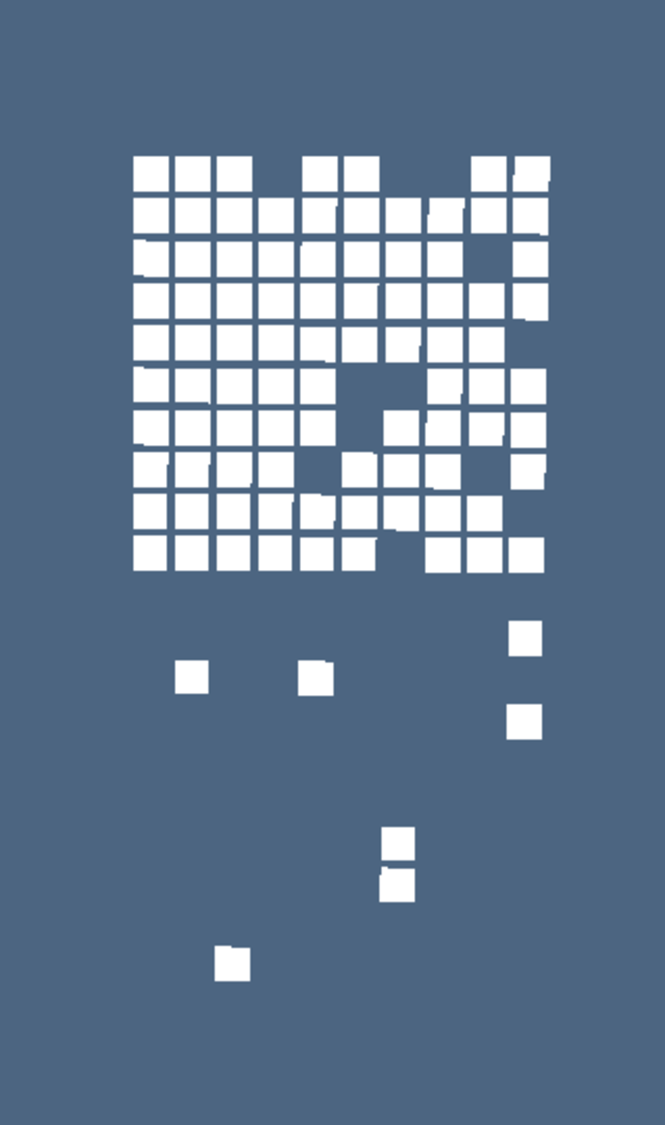
\includegraphics[height=0.3\linewidth,width=0.16\linewidth]{images/morph-chain2D1} 
   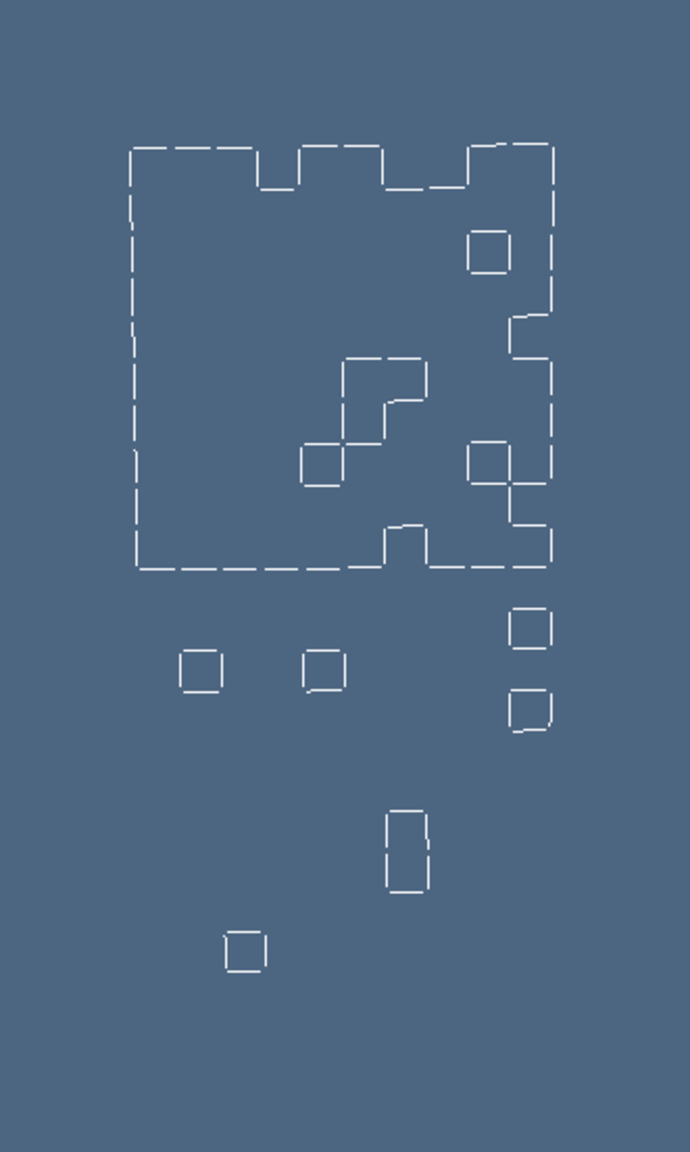
\includegraphics[height=0.3\linewidth,width=0.16\linewidth]{images/morph-chain1D1} 
   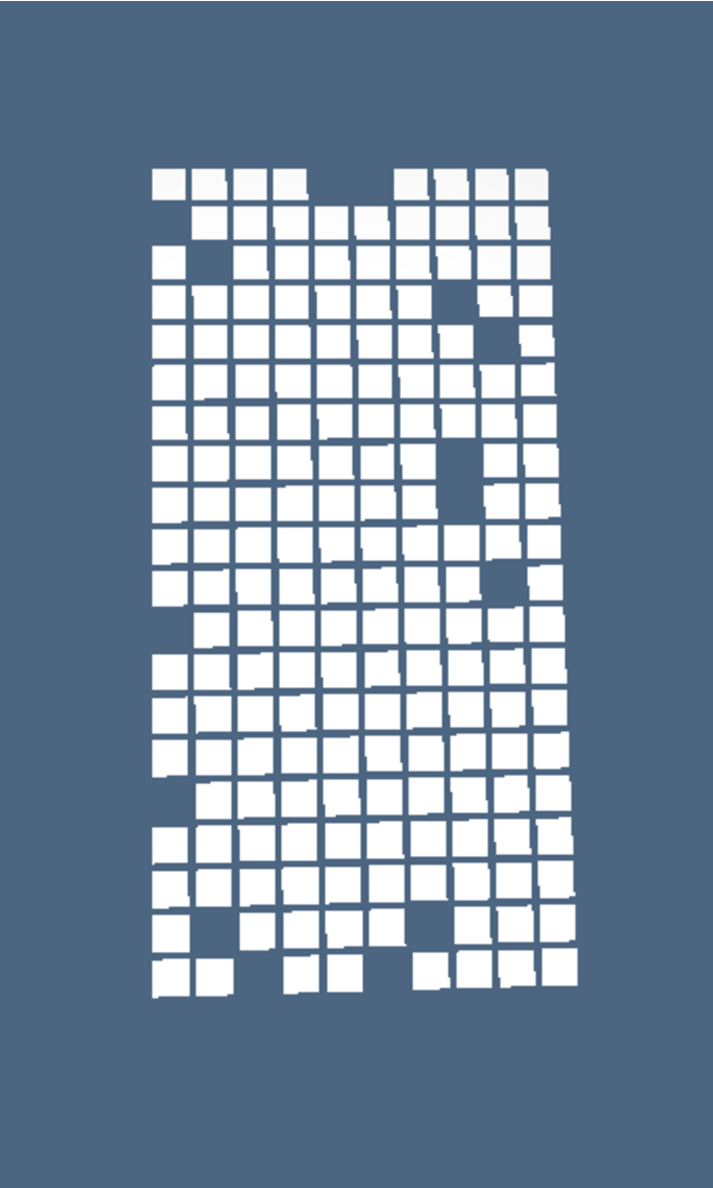
\includegraphics[height=0.3\linewidth,width=0.16\linewidth]{images/morph-chain2D2} 
   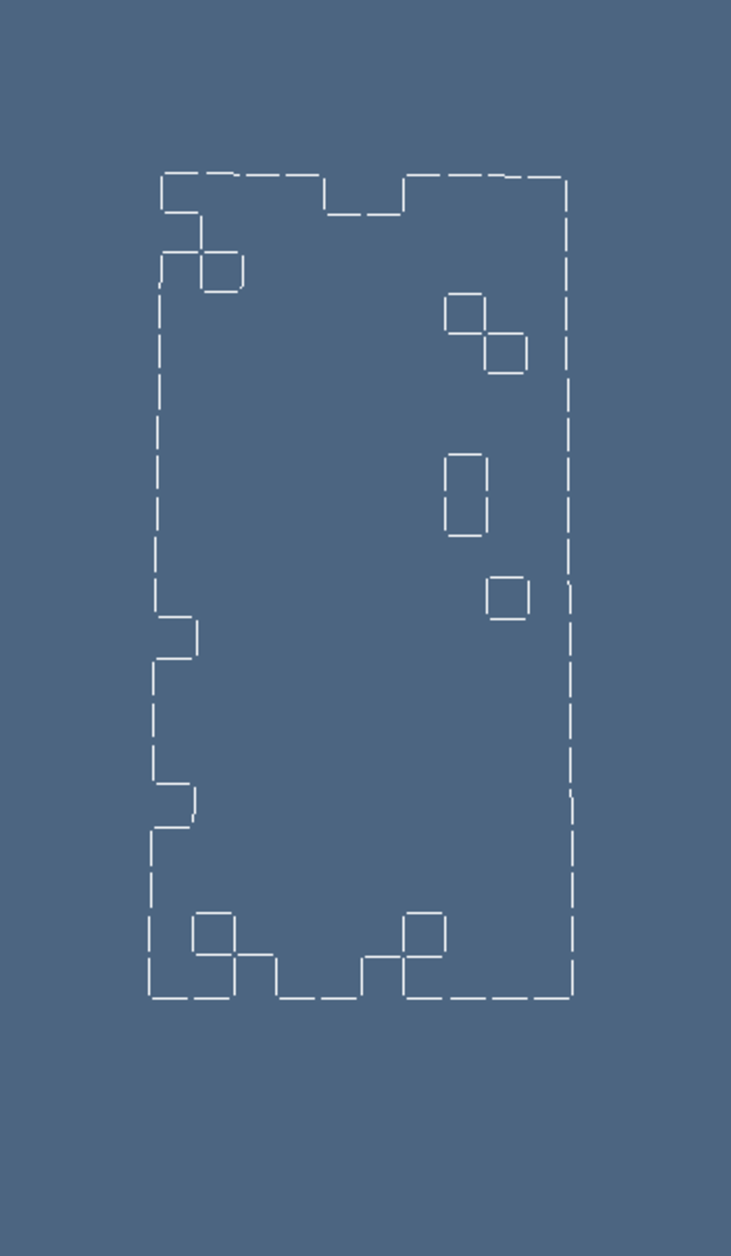
\includegraphics[height=0.3\linewidth,width=0.16\linewidth]{images/morph-chain1D2} 
   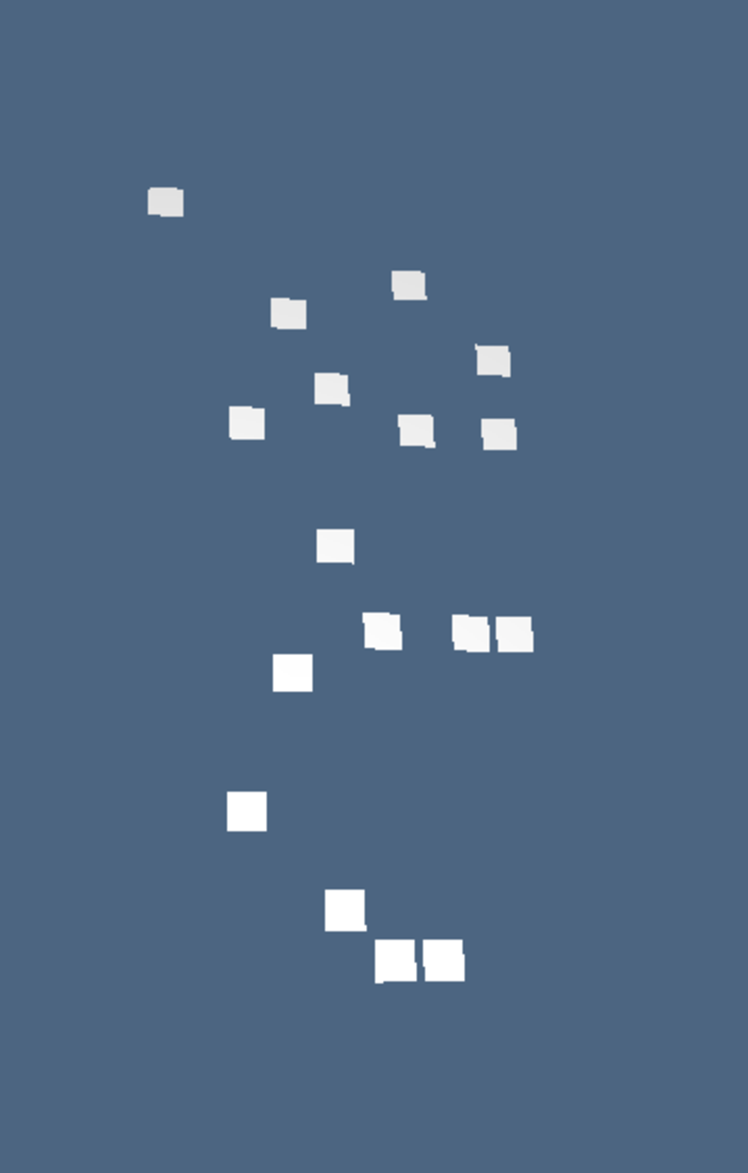
\includegraphics[height=0.3\linewidth,width=0.16\linewidth]{images/morph-chain2D3} 
   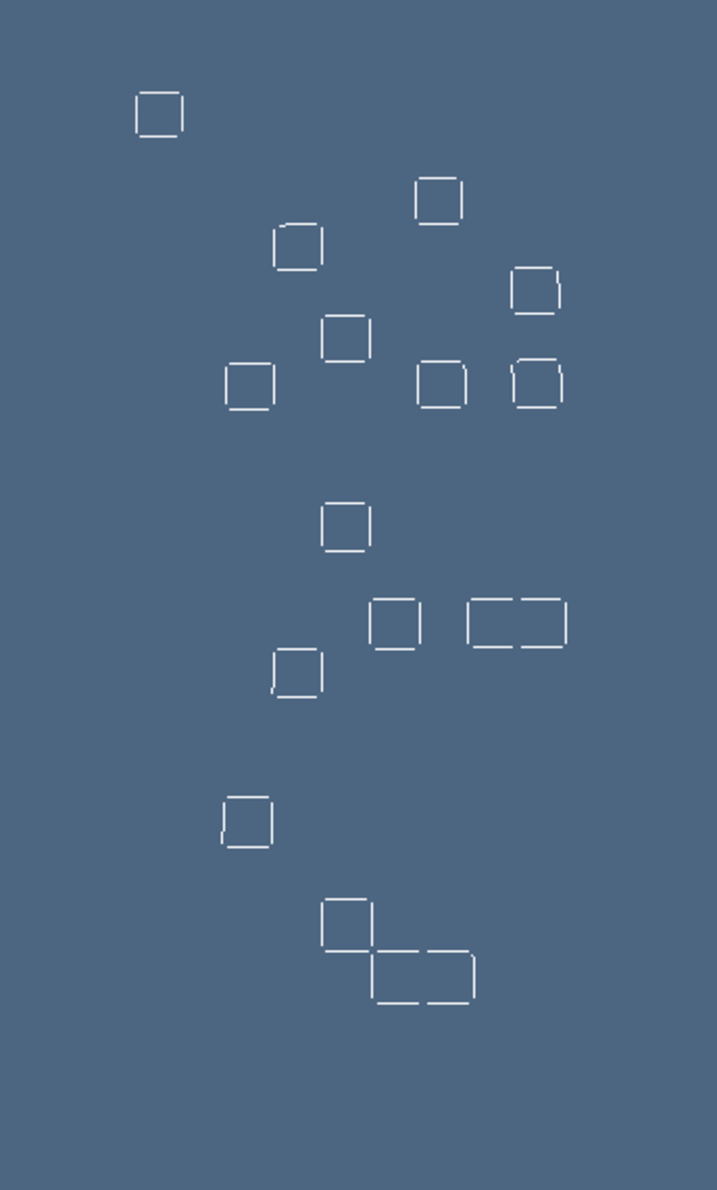
\includegraphics[height=0.3\linewidth,width=0.16\linewidth]{images/morph-chain1D3} 
   \caption{example caption}
   \label{fig:morph}
\end{figure}


\section{Exporting the \texttt{morph} module}

\paragraph{Exporting the morph module}
%-------------------------------------------------------------------------------
\begin{flushleft} \small
\begin{minipage}{\linewidth} \label{scrap10}
\protect\makebox[0ex][r]{\NWtarget{nuweb7a}{\rule{0ex}{0ex}}\hspace{1em}}\verb@"lib/py/morph.py"@\nobreak\ {\footnotesize 7a }$\equiv$
\vspace{-1ex}
\begin{list}{}{} \item
\mbox{}\verb@""" LAR implementation of morphological operators on multidimensional images."""@\\
\mbox{}\verb@@\hbox{$\langle\,$Initial import of modules\nobreak\ {\footnotesize \NWlink{nuweb7b}{7b}}$\,\rangle$}\verb@@\\
\mbox{}\verb@@\hbox{$\langle\,$Generation of random image\nobreak\ {\footnotesize \NWlink{nuweb2a}{2a}}$\,\rangle$}\verb@@\\
\mbox{}\verb@@\hbox{$\langle\,$Generation of a masking window\nobreak\ {\footnotesize \NWlink{nuweb3a}{3a}}$\,\rangle$}\verb@@\\
\mbox{}\verb@@\hbox{$\langle\,$Pyplasm visualisation of an image chain\nobreak\ {\footnotesize \NWlink{nuweb5b}{5b}}$\,\rangle$}\verb@@\\
\mbox{}\verb@@\hbox{$\langle\,$Boundary visualisation of an image chain\nobreak\ {\footnotesize \NWlink{nuweb6}{6}}$\,\rangle$}\verb@@\\
\mbox{}\verb@@{\NWsep}
\end{list}
\vspace{-2ex}
\end{minipage}\\[4ex]
\end{flushleft}
%-------------------------------------------------------------------------------

%-------------------------------------------------------------------------------
\begin{flushleft} \small
\begin{minipage}{\linewidth} \label{scrap11}
\protect\makebox[0ex][r]{\NWtarget{nuweb7b}{\rule{0ex}{0ex}}\hspace{1em}}$\langle\,$Initial import of modules\nobreak\ {\footnotesize 7b}$\,\rangle\equiv$
\vspace{-1ex}
\begin{list}{}{} \item
\mbox{}\verb@@\\
\mbox{}\verb@import scipy.misc, numpy@\\
\mbox{}\verb@from numpy.random import randint@\\
\mbox{}\verb@from pyplasm import *@\\
\mbox{}\verb@@\\
\mbox{}\verb@""" import modules from larcc/lib """@\\
\mbox{}\verb@import sys@\\
\mbox{}\verb@sys.path.insert(0, 'lib/py/')@\\
\mbox{}\verb@@\\
\mbox{}\verb@@\hbox{$\langle\,$Import the module\nobreak\ ({\footnotesize \NWtarget{nuweb7c}{7c}\label{scrap12}
 }\mbox{}\verb@largrid@ ) {\footnotesize \NWlink{nuweb8b}{8b}}$\,\rangle$}\verb@@\\
\mbox{}\verb@@\hbox{$\langle\,$Import the module\nobreak\ ({\footnotesize \NWtarget{nuweb7d}{7d}\label{scrap13}
 }\mbox{}\verb@morph@ ) {\footnotesize \NWlink{nuweb8b}{8b}}$\,\rangle$}\verb@ @\\
\mbox{}\verb@@{\NWsep}
\end{list}
\vspace{-1ex}
\footnotesize\addtolength{\baselineskip}{-1ex}
\begin{list}{}{\setlength{\itemsep}{-\parsep}\setlength{\itemindent}{-\leftmargin}}
\item \NWtxtMacroRefIn\ \NWlink{nuweb7a}{7a}\NWlink{nuweb8a}{, 8a}.
\end{list}
\end{minipage}\\[4ex]
\end{flushleft}
%-------------------------------------------------------------------------------


\section{Morphological operations examples}

\subsection{2D image masking and boundary computation}

\paragraph{Test example}

The \texttt{larcc.morph} API is used here to generate a random black and white image, with an \emph{image segment} selected and extracted by masking, then colored in middle grey, and exported to an image file.  

%------------------------------------------------------------------
\begin{flushleft} \small
\begin{minipage}{\linewidth} \label{scrap14}
\protect\makebox[0ex][r]{\NWtarget{nuweb8a}{\rule{0ex}{0ex}}\hspace{1em}}\verb@"test/py/morph/test01.py"@\nobreak\ {\footnotesize 8a }$\equiv$
\vspace{-1ex}
\begin{list}{}{} \item
\mbox{}\verb@@\hbox{$\langle\,$Initial import of modules\nobreak\ {\footnotesize \NWlink{nuweb7b}{7b}}$\,\rangle$}\verb@@\\
\mbox{}\verb@rows, columns = 100,100@\\
\mbox{}\verb@rowSize, columnSize = 10,10@\\
\mbox{}\verb@shape = (rows, columns)@\\
\mbox{}\verb@structure = (rowSize, columnSize)@\\
\mbox{}\verb@image_array = randomImage(shape, structure, 0.3)@\\
\mbox{}\verb@minPoint, maxPoint = (20,20), (40,30)@\\
\mbox{}\verb@window = minPoint, maxPoint@\\
\mbox{}\verb@segmentChain = setMaskWindow(window,image_array)@\\
\mbox{}\verb@   @\\
\mbox{}\verb@if __name__== "__main__":@\\
\mbox{}\verb@   model = visImageChain (shape,segmentChain)@\\
\mbox{}\verb@   VIEW(EXPLODE(1.2,1.2,1.2)(MKPOLS(model)))@\\
\mbox{}\verb@   model = visImageChainBoundary (shape,segmentChain)@\\
\mbox{}\verb@   VIEW(EXPLODE(1.2,1.2,1.2)(MKPOLS(model)))@\\
\mbox{}\verb@@{\NWsep}
\end{list}
\vspace{-2ex}
\end{minipage}\\[4ex]
\end{flushleft}
%------------------------------------------------------------------



%===============================================================================
\appendix
\section{Utilities}

\subsection{Importing a generic module}
First we define a parametric macro to allow the importing of \texttt{larcc} modules from the project repository \texttt{lib/py/}. When the user needs to import some project's module, she may call this macro as done in Section~\ref{sec:lar2psm}.
%------------------------------------------------------------------
\begin{flushleft} \small
\begin{minipage}{\linewidth} \label{scrap15}
\protect\makebox[0ex][r]{\NWtarget{nuweb8b}{\rule{0ex}{0ex}}\hspace{1em}}$\langle\,$Import the module\nobreak\ {\footnotesize 8b}$\,\rangle\equiv$
\vspace{-1ex}
\begin{list}{}{} \item
\mbox{}\verb@import @@1\verb@@\\
\mbox{}\verb@from @@1\verb@ import *@\\
\mbox{}\verb@@{\NWsep}
\end{list}
\vspace{-1ex}
\footnotesize\addtolength{\baselineskip}{-1ex}
\begin{list}{}{\setlength{\itemsep}{-\parsep}\setlength{\itemindent}{-\leftmargin}}
\item \NWtxtMacroRefIn\ \NWlink{nuweb7b}{7b}\NWlink{nuweb8c}{, 8c}.
\end{list}
\end{minipage}\\[4ex]
\end{flushleft}
%------------------------------------------------------------------

\paragraph{Importing a module} A function used to import a generic \texttt{lacccc} module within the current environment is also useful.
%------------------------------------------------------------------
\begin{flushleft} \small
\begin{minipage}{\linewidth} \label{scrap16}
\protect\makebox[0ex][r]{\NWtarget{nuweb8c}{\rule{0ex}{0ex}}\hspace{1em}}$\langle\,$Function to import a generic module\nobreak\ {\footnotesize 8c}$\,\rangle\equiv$
\vspace{-1ex}
\begin{list}{}{} \item
\mbox{}\verb@def importModule(moduleName):@\\
\mbox{}\verb@   @\hbox{$\langle\,$Import the module\nobreak\ ({\footnotesize \NWtarget{nuweb8d}{8d}\label{scrap17}
 }\mbox{}\verb@moduleName@ ) {\footnotesize \NWlink{nuweb8b}{8b}}$\,\rangle$}\verb@@\\
\mbox{}\verb@@{\NWsep}
\end{list}
\vspace{-1ex}
\footnotesize\addtolength{\baselineskip}{-1ex}
\begin{list}{}{\setlength{\itemsep}{-\parsep}\setlength{\itemindent}{-\leftmargin}}
\item {\NWtxtMacroNoRef}.
\end{list}
\end{minipage}\\[4ex]
\end{flushleft}
%------------------------------------------------------------------


\bibliographystyle{amsalpha}
\bibliography{morph}

\end{document}
